% Options for packages loaded elsewhere
% Options for packages loaded elsewhere
\PassOptionsToPackage{unicode}{hyperref}
\PassOptionsToPackage{hyphens}{url}
\PassOptionsToPackage{dvipsnames,svgnames,x11names}{xcolor}
%
\documentclass[
  british,
  a4paper,
]{article}
\usepackage{xcolor}
\usepackage{amsmath,amssymb}
\setcounter{secnumdepth}{-\maxdimen} % remove section numbering
\usepackage{iftex}
\ifPDFTeX
  \usepackage[T1]{fontenc}
  \usepackage[utf8]{inputenc}
  \usepackage{textcomp} % provide euro and other symbols
\else % if luatex or xetex
  \usepackage{unicode-math} % this also loads fontspec
  \defaultfontfeatures{Scale=MatchLowercase}
  \defaultfontfeatures[\rmfamily]{Ligatures=TeX,Scale=1}
\fi
\usepackage{lmodern}
\ifPDFTeX\else
  % xetex/luatex font selection
\fi
% Use upquote if available, for straight quotes in verbatim environments
\IfFileExists{upquote.sty}{\usepackage{upquote}}{}
\IfFileExists{microtype.sty}{% use microtype if available
  \usepackage[]{microtype}
  \UseMicrotypeSet[protrusion]{basicmath} % disable protrusion for tt fonts
}{}
\makeatletter
\@ifundefined{KOMAClassName}{% if non-KOMA class
  \IfFileExists{parskip.sty}{%
    \usepackage{parskip}
  }{% else
    \setlength{\parindent}{0pt}
    \setlength{\parskip}{6pt plus 2pt minus 1pt}}
}{% if KOMA class
  \KOMAoptions{parskip=half}}
\makeatother
% Make \paragraph and \subparagraph free-standing
\makeatletter
\ifx\paragraph\undefined\else
  \let\oldparagraph\paragraph
  \renewcommand{\paragraph}{
    \@ifstar
      \xxxParagraphStar
      \xxxParagraphNoStar
  }
  \newcommand{\xxxParagraphStar}[1]{\oldparagraph*{#1}\mbox{}}
  \newcommand{\xxxParagraphNoStar}[1]{\oldparagraph{#1}\mbox{}}
\fi
\ifx\subparagraph\undefined\else
  \let\oldsubparagraph\subparagraph
  \renewcommand{\subparagraph}{
    \@ifstar
      \xxxSubParagraphStar
      \xxxSubParagraphNoStar
  }
  \newcommand{\xxxSubParagraphStar}[1]{\oldsubparagraph*{#1}\mbox{}}
  \newcommand{\xxxSubParagraphNoStar}[1]{\oldsubparagraph{#1}\mbox{}}
\fi
\makeatother


\usepackage{longtable,booktabs,array}
\newcounter{none} % for unnumbered tables
\usepackage{calc} % for calculating minipage widths
% Correct order of tables after \paragraph or \subparagraph
\usepackage{etoolbox}
\makeatletter
\patchcmd\longtable{\par}{\if@noskipsec\mbox{}\fi\par}{}{}
\makeatother
% Allow footnotes in longtable head/foot
\IfFileExists{footnotehyper.sty}{\usepackage{footnotehyper}}{\usepackage{footnote}}
\makesavenoteenv{longtable}
\usepackage{graphicx}
\makeatletter
\newsavebox\pandoc@box
\newcommand*\pandocbounded[1]{% scales image to fit in text height/width
  \sbox\pandoc@box{#1}%
  \Gscale@div\@tempa{\textheight}{\dimexpr\ht\pandoc@box+\dp\pandoc@box\relax}%
  \Gscale@div\@tempb{\linewidth}{\wd\pandoc@box}%
  \ifdim\@tempb\p@<\@tempa\p@\let\@tempa\@tempb\fi% select the smaller of both
  \ifdim\@tempa\p@<\p@\scalebox{\@tempa}{\usebox\pandoc@box}%
  \else\usebox{\pandoc@box}%
  \fi%
}
% Set default figure placement to htbp
\def\fps@figure{htbp}
\makeatother



\ifLuaTeX
\usepackage[bidi=basic,shorthands=off]{babel}
\else
\usepackage[bidi=default,shorthands=off]{babel}
\fi
\ifLuaTeX
  \usepackage{selnolig} % disable illegal ligatures
\fi


\setlength{\emergencystretch}{3em} % prevent overfull lines

\providecommand{\tightlist}{%
  \setlength{\itemsep}{0pt}\setlength{\parskip}{0pt}}



 


\makeatletter
\@ifpackageloaded{tcolorbox}{}{\usepackage[skins,breakable]{tcolorbox}}
\@ifpackageloaded{fontawesome5}{}{\usepackage{fontawesome5}}
\definecolor{quarto-callout-color}{HTML}{909090}
\definecolor{quarto-callout-note-color}{HTML}{0758E5}
\definecolor{quarto-callout-important-color}{HTML}{CC1914}
\definecolor{quarto-callout-warning-color}{HTML}{EB9113}
\definecolor{quarto-callout-tip-color}{HTML}{00A047}
\definecolor{quarto-callout-caution-color}{HTML}{FC5300}
\definecolor{quarto-callout-color-frame}{HTML}{acacac}
\definecolor{quarto-callout-note-color-frame}{HTML}{4582ec}
\definecolor{quarto-callout-important-color-frame}{HTML}{d9534f}
\definecolor{quarto-callout-warning-color-frame}{HTML}{f0ad4e}
\definecolor{quarto-callout-tip-color-frame}{HTML}{02b875}
\definecolor{quarto-callout-caution-color-frame}{HTML}{fd7e14}
\makeatother
\makeatletter
\@ifpackageloaded{caption}{}{\usepackage{caption}}
\AtBeginDocument{%
\ifdefined\contentsname
  \renewcommand*\contentsname{Table of contents}
\else
  \newcommand\contentsname{Table of contents}
\fi
\ifdefined\listfigurename
  \renewcommand*\listfigurename{List of Figures}
\else
  \newcommand\listfigurename{List of Figures}
\fi
\ifdefined\listtablename
  \renewcommand*\listtablename{List of Tables}
\else
  \newcommand\listtablename{List of Tables}
\fi
\ifdefined\figurename
  \renewcommand*\figurename{Figure}
\else
  \newcommand\figurename{Figure}
\fi
\ifdefined\tablename
  \renewcommand*\tablename{Table}
\else
  \newcommand\tablename{Table}
\fi
}
\@ifpackageloaded{float}{}{\usepackage{float}}
\floatstyle{ruled}
\@ifundefined{c@chapter}{\newfloat{codelisting}{h}{lop}}{\newfloat{codelisting}{h}{lop}[chapter]}
\floatname{codelisting}{Listing}
\newcommand*\listoflistings{\listof{codelisting}{List of Listings}}
\makeatother
\makeatletter
\makeatother
\makeatletter
\@ifpackageloaded{caption}{}{\usepackage{caption}}
\@ifpackageloaded{subcaption}{}{\usepackage{subcaption}}
\makeatother
\usepackage{bookmark}
\IfFileExists{xurl.sty}{\usepackage{xurl}}{} % add URL line breaks if available
\urlstyle{same}
% fallback for those not using the hyperref driver hyperxmp:
\makeatletter
\@ifundefined{xmpquote}{\newcommand{\xmpquote}[1]{#1}}{}
\makeatother
\hypersetup{
  pdftitle={Signal extraction across tens of thousands of series pairs},
  pdfauthor={Carlos Galindo},
  pdflang={en-GB},
  colorlinks=true,
  linkcolor={blue},
  filecolor={Maroon},
  citecolor={Blue},
  urlcolor={Blue},
  pdfcreator={LaTeX via pandoc}}


\title{Signal extraction across tens of thousands of series pairs}
\usepackage{etoolbox}
\makeatletter
\providecommand{\subtitle}[1]{% add subtitle to \maketitle
  \apptocmd{\@title}{\par {\large #1 \par}}{}{}
}
\makeatother
\subtitle{A pipeline that decomposes thousands of price and activity
series and measures how every pair moves together, without ever
repeating a pair}
\author{Carlos Galindo}
\date{}
\begin{document}
\maketitle


\begin{tcolorbox}[enhanced jigsaw, arc=.35mm, bottomrule=.15mm, breakable, colback=white, colframe=quarto-callout-note-color-frame, left=2mm, leftrule=.75mm, opacityback=0, rightrule=.15mm, toprule=.15mm]

\vspace{-3mm}\textbf{At a glance}\vspace{3mm}

\begin{itemize}
\tightlist
\item
  \textbf{Question.} Which economic series share a common cyclical
  signal, once seasonality and trend are removed, when the number of
  candidate pairs is far too large to inspect by hand or to compute in
  one run?
\item
  \textbf{Approach.} Decompose each series into trend, seasonal and
  residual parts, measure how each pair of residuals moves together
  across frequencies, and run the work in resumable batches with a
  persistent record of every pair already analysed.
\item
  \textbf{Finding.} The system analysed more than 72,000 pairs of
  economic series in 2025, drawn from a universe of roughly 82 million
  possible pairs, and kept every result queryable.
\item
  \textbf{Why it matters.} Co-movement screens are only credible when
  the search is wide, repeatable and explicit about what it covers. This
  is the machinery for that.
\end{itemize}

\end{tcolorbox}

\subsection{The question}\label{the-question}

Macroeconomists usually study co-movement one pair at a time. Does a
producer price index lead a consumer price index? Do two countries'
price components share a business-cycle rhythm? Each answer is a small,
careful piece of work. The trouble is that the interesting relationships
are rarely the ones we thought to test first. A wide screen across a
large collection of series can surface pairs worth a closer look, but
only if it is run consistently, so that a strong result is not simply
the best of an unrecorded, uneven search.

The collection I worked with was large: 12,804 unique series identifiers
from a licensed macroeconomic database, covering price and activity
measures for two large economies. Twelve thousand series imply about 82
million distinct pairs. No single run can cover that, and a naive
approach of drawing random pairs again and again has two defects. It
wastes effort on pairs it has already seen, and it leaves no record of
what has and has not been searched, so any claim of the form ``the most
coherent pairs are these'' cannot be interpreted.

The goal was therefore twofold: a sound method for pulling a signal out
of each series and comparing pairs, and an engineering layer that lets
that method run at volume, resume after interruption, and never silently
repeat itself.

\subsection{Approach}\label{approach}

\subsubsection{Step one: remove what is not the
signal}\label{step-one-remove-what-is-not-the-signal}

Raw economic series mix at least three things: a slow-moving trend, a
regular calendar pattern, and the remainder, which carries the cyclical
and shock-driven movement an economist usually cares about. Comparing
two raw series mostly compares their trends and their calendars, which
is how spurious correlation arises. So each series is decomposed into
trend, seasonal and residual components, using an additive decomposition
with a twelve-period cycle for monthly data. The trend is a centred
moving average, which cannot be computed for the first and last few
months, so those ends are filled rather than extrapolated and every
series keeps its full length.

\subsubsection{Step two: measure co-movement by
frequency}\label{step-two-measure-co-movement-by-frequency}

For each pair, the residual components are compared in the frequency
domain. Spectral coherence is the frequency-domain analogue of a squared
correlation: at each cycle length it says how much of the movement in
one series is linearly accounted for by the other. Reading it by
frequency matters. Two price series can be tightly linked at medium-run
cycles and unrelated at short ones, and a single correlation coefficient
averages those stories together. The analysis also records gain (how
strongly one series responds to the other at each frequency) and phase
(which one moves first). The summary kept for every pair is the average
coherence, the maximum coherence and the frequency at which that maximum
occurs.

\subsubsection{Step three: make the search wide, uneven-proof and
resumable}\label{step-three-make-the-search-wide-uneven-proof-and-resumable}

Three design choices turn the method into infrastructure.

\begin{itemize}
\tightlist
\item
  \textbf{Stratified sampling.} Series are drawn across their
  statistical release categories rather than uniformly, so that a
  handful of very large categories do not crowd out everything else.
\item
  \textbf{A persistent record of analysed pairs.} Every pair is stored
  once, with its two identifiers in a fixed order, a timestamp, a run
  label, the release categories of both series and a success flag. The
  record is partitioned by date and by a hashed bucket so that lookups
  stay fast as it grows. A pair already in the record is never drawn
  again, in any later run. If a run is interrupted, writes are arranged
  so that no pair is lost or counted twice.
\item
  \textbf{Batch parallelism with a fallback.} Pairs are processed in
  parallel batches, with results written in bulk to limit input and
  output overhead. The coherence step was later redesigned to use
  graphics-processor acceleration where available, and to fall back to
  ordinary processing where it is not, with the same outputs either way.
\end{itemize}

The averaged coherence of each pair is also held in a lower-triangular
matrix, in the same way a correlation matrix is stored, so that the full
pairwise picture can be queried or exported as the search grows.

\subsubsection{How it was checked}\label{how-it-was-checked}

The validation design was practical. The method was first developed on a
small sample, and the scaled version was specified to keep the same
output structure as the original, with coherence results required to be
numerically stable and with a check that no pair is ever sampled twice.
Because the record guarantees uniqueness, the count of analysed pairs
can be audited directly: it is meant to be read from the record itself,
not reconstructed from run logs.

\subsection{What the work shows}\label{what-the-work-shows}

The headline result is one of scale and coverage. The system analysed
more than 72,000 pairs of economic series in 2025. Against roughly 82
million possible pairs, that is a little under one tenth of one per cent
of the space. The right reading is not that the search is nearly
complete. It is that a wide, recorded and extendable screen now exists,
and that its coverage can be stated exactly.

The figures below use simulated data built to share the structure of the
real analysis: monthly series, a twelve-period seasonal cycle, residual
components compared by frequency, and a large pool of candidate pairs.
They illustrate how the method behaves; they are not the project's
results.

\begin{figure}

\centering{

\pandocbounded{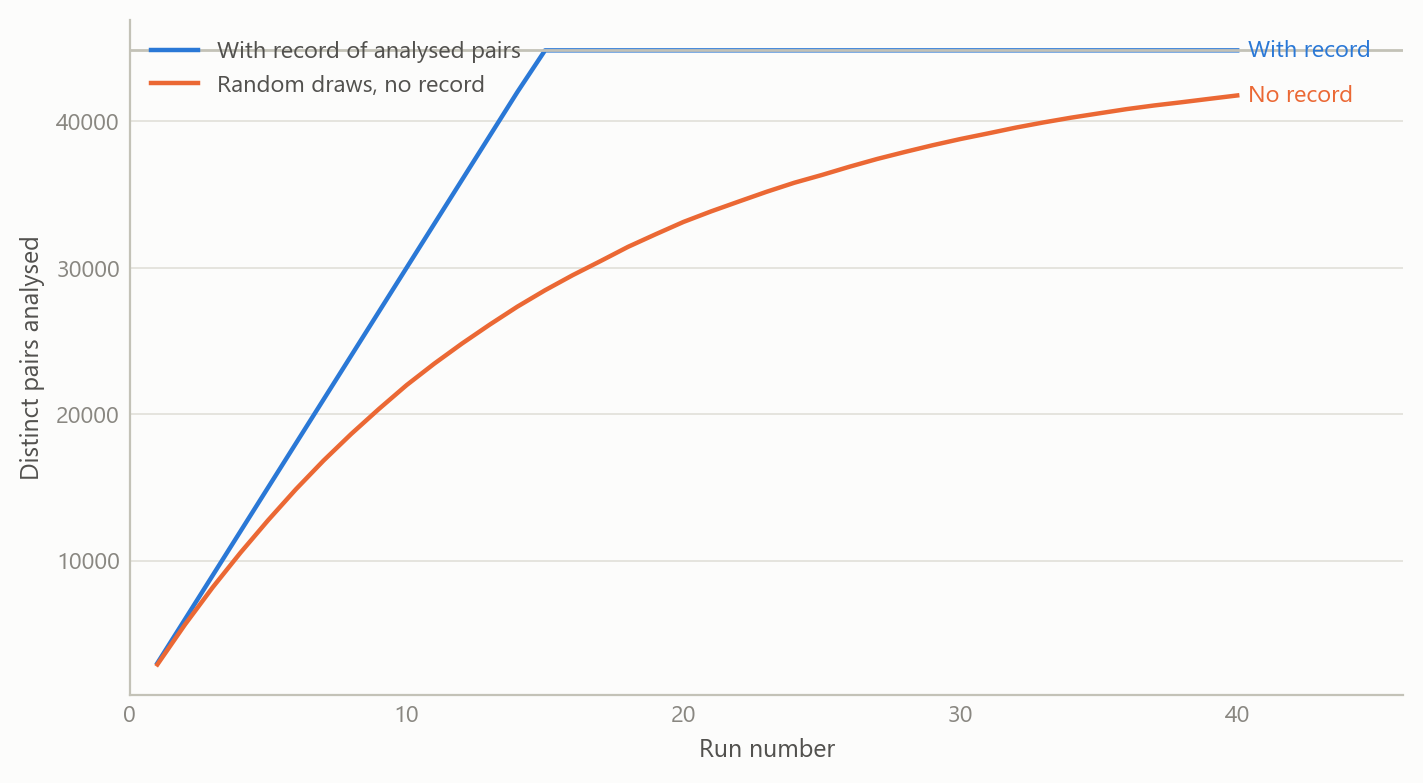
\includegraphics[keepaspectratio]{index_files/figure-latex/fig-coverage-output-1.png}}

}

\caption{\label{fig-coverage}Cumulative number of distinct pairs
analysed, with and without a persistent record, in a scaled-down
universe of 300 series (simulated data).}

\end{figure}%

Without a record, repeated random draws re-analyse pairs they have
already seen, and the shortfall against the recorded search is large for
most of the run sequence, until the recorded search has exhausted the
space. At the real scale the gap matters less in any one run, because
the space is so large, but the inability to say what has been covered
does not go away.

\begin{figure}

\centering{

\pandocbounded{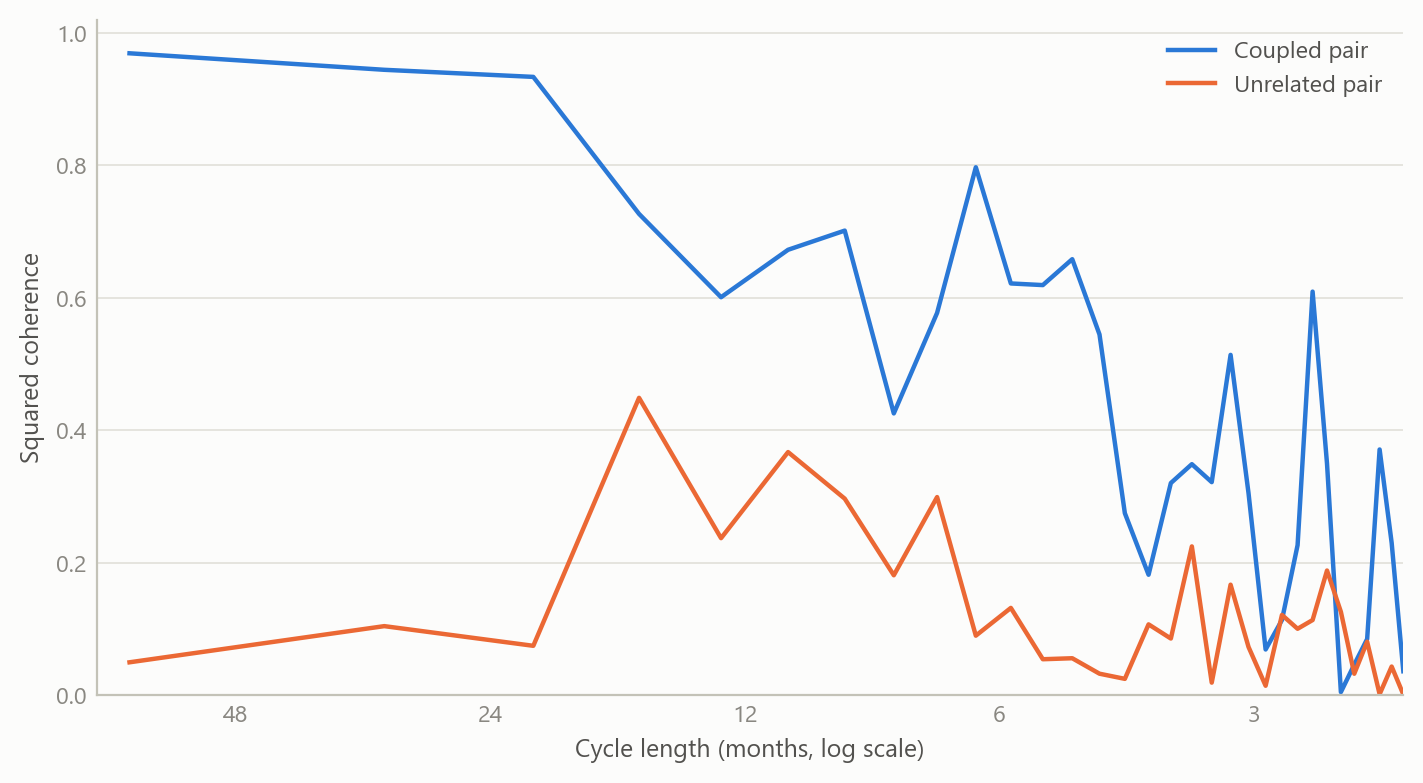
\includegraphics[keepaspectratio]{index_files/figure-latex/fig-coherence-output-1.png}}

}

\caption{\label{fig-coherence}Coherence by cycle length for a coupled
pair and an unrelated pair of monthly residual series, 300 months
(simulated data).}

\end{figure}%

The coupled pair shares a slow cycle, so its coherence is high at long
cycle lengths and falls away at short ones, while the unrelated pair
sits low throughout. An averaged correlation would blur this into a
single moderate number. Keeping the frequency detail is what lets a
screen separate a medium-run link from noise.

\begin{figure}

\centering{

\pandocbounded{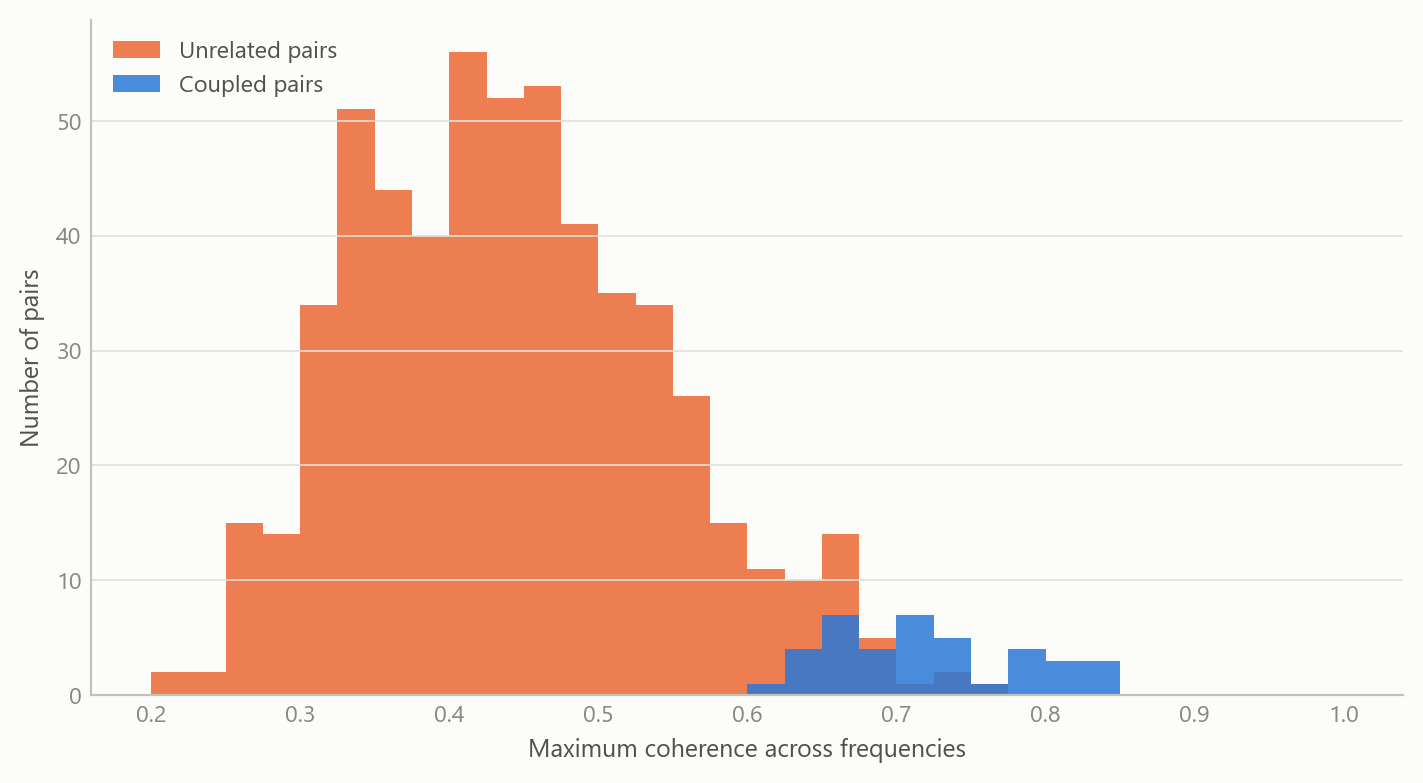
\includegraphics[keepaspectratio]{index_files/figure-latex/fig-screen-output-1.png}}

}

\caption{\label{fig-screen}Maximum coherence across 600 simulated pairs,
5 per cent of which share a common cycle (simulated data).}

\end{figure}%

When a large share of unrelated pairs is screened, some will show high
maximum coherence by chance, and the coupled pairs overlap with the
upper tail of that crowd. This is the practical reason the search must
be recorded: the number of pairs examined is part of how any single high
value should be read.

\subsection{Insights}\label{insights}

\begin{enumerate}
\def\labelenumi{\arabic{enumi}.}
\tightlist
\item
  \textbf{Scale changes what counts as evidence.} With 82 million
  possible pairs, a strong coherence value is only meaningful alongside
  the number of pairs that were searched. Recording coverage is a
  statistical requirement, not housekeeping.
\item
  \textbf{Frequency detail is the point.} Co-movement that lives at
  medium-run cycle lengths is invisible in a single correlation.
  Decomposing first and comparing by frequency afterwards removes the
  trend and calendar artefacts that inflate naive comparisons.
\item
  \textbf{Uniqueness has to be enforced, not hoped for.} A persistent
  record of analysed pairs, with an ordering rule for the two
  identifiers, turned ``never repeat a pair'' from an intention into a
  property of the system.
\item
  \textbf{Design for interruption.} Long jobs fail. Atomic writes, bulk
  batching and a fallback path meant that a failed run cost one batch
  rather than the whole search.
\item
  \textbf{Early planning documents were worth keeping.} The written
  plans for tracking, storage and the pairwise matrix made the later
  acceleration work a refactor rather than a rewrite.
\end{enumerate}

\subsection{Scope and next steps}\label{scope-and-next-steps}

The screen is built to search a very large space of macroeconomic series
for pairs that move together at particular frequencies, as a first stage
that surfaces candidates for economic study. The search is stratified,
so it samples the space rather than enumerating it, and long runs are
protected so that a failure costs one batch, not the whole search.

The natural extensions are two. First, a second stage for pairs of
interest: stability across sub-periods, a correction for the number of
pairs searched, and an economic story. Second, a published simulated
benchmark on which the full screen, including its multiple-testing
correction, can be demonstrated end to end.

The source data are licensed, so the series and the ranked list of
strongest pairs are not reproduced here; the results can be discussed on
request.

\subsection{About the evidence}\label{about-the-evidence}

The project ran in 2025, during a period of independent research. The
scale figures (the number of series, the size of the pair space and the
number of pairs analysed) come from the project's planning documents and
my record of the work. The decomposition and coherence design described
above is what the infrastructure implements. All figures on this page
are simulated, built to share the structure of the real analysis
(monthly series, a twelve-period seasonal cycle, residual comparison by
frequency and a large pool of candidate pairs).

Figures and tables marked \emph{simulated} are generated from simulated
data built to share the structure of the analysis (its variables,
horizons and frequencies). They show how each method works and what its
output looks like. Results stated in the text, and figures that give a
source, are the project's own. Methods are described at the level of a
methods section. Code and data pipelines are not reproduced here.




\end{document}
